\documentclass[journal,12pt,twocolumn]{IEEEtran}
%

\usepackage{setspace}
\usepackage{gensymb}
\singlespacing

\usepackage{amsmath}
\usepackage{amsthm}
\usepackage{txfonts}
\usepackage{cite}
\usepackage{enumitem}
\usepackage{mathtools}
\usepackage{listings}
    \usepackage{color}                                            %%
    \usepackage{array}                                            %%
    \usepackage{longtable}                                        %%
    \usepackage{calc}                                             %%
    \usepackage{multirow}                                         %%
    \usepackage{hhline}                                           %%
    \usepackage{ifthen}                                           %%
  %optionally (for landscape tables embedded in another document): %%
    \usepackage{lscape}     
\usepackage{multicol}
\usepackage{chngcntr}
\renewcommand\thesection{\arabic{section}}
\renewcommand\thesubsection{\thesection.\arabic{subsection}}
\renewcommand\thesubsubsection{\thesubsection.\arabic{subsubsection}}

\renewcommand\thesectiondis{\arabic{section}}
\renewcommand\thesubsectiondis{\thesectiondis.\arabic{subsection}}
\renewcommand\thesubsubsectiondis{\thesubsectiondis.\arabic{subsubsection}}

% correct bad hyphenation here
\hyphenation{op-tical net-works semi-conduc-tor}
\def\inputGnumericTable{}                                 %%

\lstset{
%language=C,
frame=single, 
breaklines=true,
columns=fullflexible
}

\begin{document}
%


\newtheorem{theorem}{Theorem}[section]
\newtheorem{problem}{Problem}
\newtheorem{proposition}{Proposition}[section]
\newtheorem{lemma}{Lemma}[section]
\newtheorem{corollary}[theorem]{Corollary}
\newtheorem{example}{Example}[section]
\newtheorem{definition}[problem]{Definition}
\newcommand{\BEQA}{\begin{eqnarray}}
\newcommand{\EEQA}{\end{eqnarray}}
\newcommand{\define}{\stackrel{\triangle}{=}}
\bibliographystyle{IEEEtran}
\providecommand{\mbf}{\mathbf}
\providecommand{\pr}[1]{\ensuremath{\Pr\left(#1\right)}}
\providecommand{\qfunc}[1]{\ensuremath{Q\left(#1\right)}}
\providecommand{\sbrak}[1]{\ensuremath{{}\left[#1\right]}}
\providecommand{\lsbrak}[1]{\ensuremath{{}\left[#1\right.}}
\providecommand{\rsbrak}[1]{\ensuremath{{}\left.#1\right]}}
\providecommand{\brak}[1]{\ensuremath{\left(#1\right)}}
\providecommand{\lbrak}[1]{\ensuremath{\left(#1\right.}}
\providecommand{\rbrak}[1]{\ensuremath{\left.#1\right)}}
\providecommand{\cbrak}[1]{\ensuremath{\left\{#1\right\}}}
\providecommand{\lcbrak}[1]{\ensuremath{\left\{#1\right.}}
\providecommand{\rcbrak}[1]{\ensuremath{\left.#1\right\}}}
\theoremstyle{remark}
\newtheorem{rem}{Remark}
\newcommand{\sgn}{\mathop{\mathrm{sgn}}}
\providecommand{\abs}[1]{\left\vert#1\right\vert}
\providecommand{\res}[1]{\Res\displaylimits_{#1}} 
\providecommand{\norm}[1]{\left\lVert#1\right\rVert}
\providecommand{\mtx}[1]{\mathbf{#1}}
\providecommand{\mean}[1]{E\left[ #1 \right]}
\providecommand{\fourier}{\overset{\mathcal{F}}{ \rightleftharpoons}}
\providecommand{\system}{\overset{\mathcal{H}}{ \longleftrightarrow}}


\newcommand{\myvec}[1]{\ensuremath{\begin{pmatrix}#1\end{pmatrix}}}
\newcommand{\cmyvec}[1]{\ensuremath{\begin{pmatrix*}[c]#1\end{pmatrix*}}}
\newcommand{\mydet}[1]{\ensuremath{\begin{vmatrix}#1\end{vmatrix}}}
\newcommand{\proj}[2]{\textbf{proj}_{\vec{#1}}\vec{#2}}
\let\StandardTheFigure\thefigure
\let\vec\mathbf
\title{
ASSIGNMENT 2
}
\author{Gayathri S}
	

\maketitle
\renewcommand{\thefigure}{\theenumi}
\renewcommand{\thetable}{\theenumi}
  
\section{Linear forms 2.11}

Which of the following pairs of linear equations has a unique solution,no solution,or infinitely many solutions?
\begin{enumerate}
    \item $\myvec{3\\-5}\vec{x}$=20 and $\myvec{6\\-10}\vec{x}$=40
    \item $\myvec{1\\-3}\vec{x}$=7 and $\myvec{3\\-3}\vec{x}$=15
\end{enumerate}
%
%
\section{Solution}
\begin{enumerate}
    \item Given $\myvec{3\\-5}\vec{x}$=20 and $\myvec{6\\-10}\vec{x}$=40.The above equations can be expressed as a matrix equation.
    \begin{align}
\label{eq:1}
  \myvec{3&-5\\6&-10}\vec{x} &= \myvec{20\\40}
\end{align}
The augmented matrix for the above equation
is row reduced as follows
\begin{align}
    \myvec{3&-5&20\\6&-10&40}\xleftrightarrow{R_2\leftarrow R_2 -2R_1}\myvec{3&-5&20\\0&0&0} \label{eq:(2)}
\end{align}
The rank of\begin{equation} 
\myvec{3&-5\\6&-10} = 1
\end{equation} and the rank of
\begin{equation} 
\myvec{3&-5&20\\6&-10&40} = 1
\end{equation}from \ref{eq:(2)} .
\begin{align}
    \therefore rank \myvec{3&-5\\6&-10} &= rank\myvec{3&-5&20\\6&-10&40}\\
    &=1 < dim\myvec{3&-5\\6&-10}=2
\end{align}
$\Longrightarrow$ \ref{eq:1} has infinitely many solutions.
Fig\ref{fig:1} shows that the lines are the same.
\numberwithin{figure}{section}
\begin{figure}[ht] 
    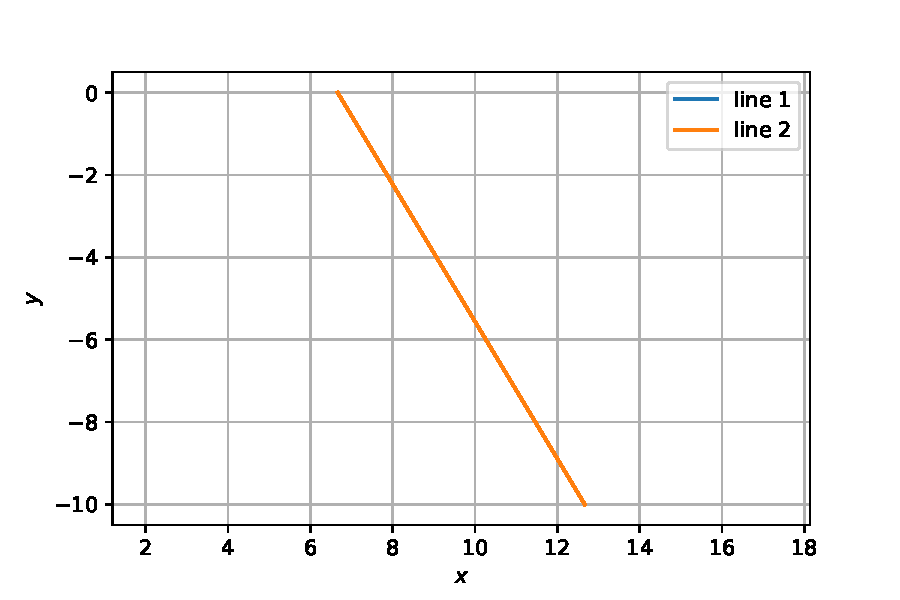
\includegraphics[width= \columnwidth]{assignment2c.pdf}
    \caption{Lines coincide:infinitely many solutions}
    \label{fig:1}
\end{figure}


    \item Given $\myvec{1\\-3}\vec{x}$=7 and $\myvec{3\\-3}\vec{x}$=15.
    The above equations can be expressed as a matrix equation.
    \begin{align}
\label{eq:7}
  \myvec{1&-3\\3&-3}\vec{x} &= \myvec{7\\15}
\end{align}
The augmented matrix for the above equation
is row reduced as follows
\begin{align}
    \myvec{1&-3&7\\3&-3&15}\xleftrightarrow{R_2\leftarrow R_2 -R_1}\myvec{1&-3&7\\2&0&8} 
    \\ 
    \myvec{1&-3&7\\2&0&8}\xleftrightarrow{R_2\leftarrow R_2 -2R_1}\myvec{1&-3&7\\0&6&-6} 
    \\
    \myvec{1&-3&7\\0&6&-6}\xleftrightarrow{R_1\leftarrow R_1 +\frac{R_2}{2}}\myvec{1&0&4\\0&6&-6} 
\\ \myvec{1&0&4\\0&6&-6}\xleftrightarrow{R_2\leftarrow\frac{R_2}{6}}\myvec{1&0&4\\0&1&-1} \label{eq:11}\end{align} 
\begin{align}
 \Longrightarrow \vec{x}&=\myvec{4\\-1}
\end{align} is a solution of \ref{eq:7}.
The rank of
\begin{equation} 
\myvec{1&-3\\3&-3} = 2
\end{equation}
and the rank of
\begin{equation} 
\myvec{1&-3&7\\3&-3&15} = 2
\end{equation}from \ref{eq:11} .
\begin{align}
    \therefore rank \myvec{3&-5\\6&-10} &= rank\myvec{3&-5&20\\6&-10&40}\\
    &=dim\myvec{3&-5\\6&-10}=2
\end{align}
$\Longrightarrow$ \ref{eq:7} has a unique solution, $\vec{x}=\myvec{4\\-1}$
Fig\ref{fig:2} shows that the lines intersect only at one point.

\numberwithin{figure}{section}
\begin{figure}[ht]
    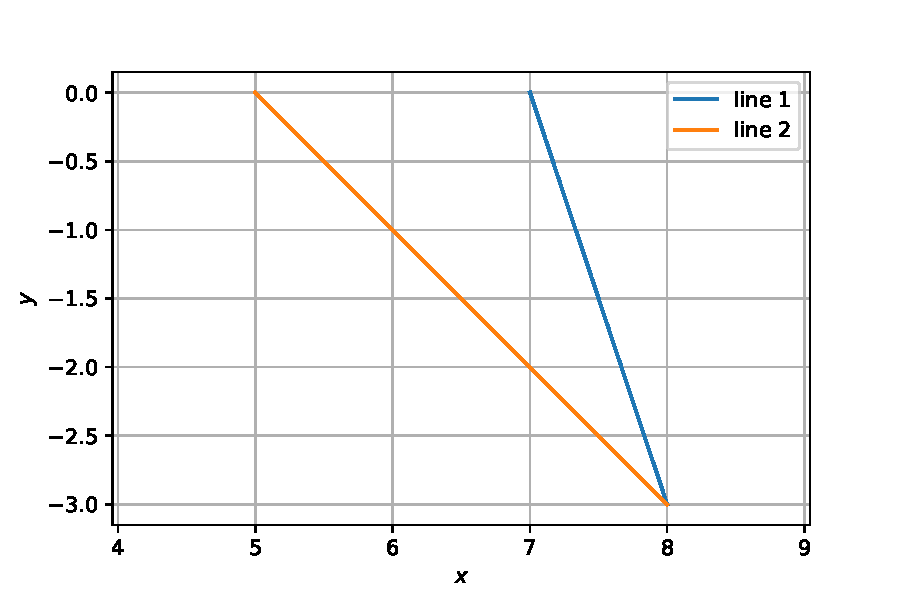
\includegraphics[width= \columnwidth]{assignment2d.pdf}
    \caption{Lines intersecting only at one point:unique solution}
    \label{fig:2}
\end{figure}
\end{enumerate}
\end{document}
